\documentclass[t]{beamer}

\usetheme{TuringLight}
%\usetheme{TuringDark}
\usepackage{svg}
\usepackage{amsmath}

% Presentation data
\title{Creating a well-being data layer using open source data}





% Uncomment any of these lines below to set custom size for each of the font sizes.
% The default value is shown in the comment.
%\setlength{\titlefontsize}{6.875\basefontsize}
%\setlength{\subtitlefontsize}{4.375\basefontsize}
%\setlength{\frametitlesize}{2.625\basefontsize}
%\setlength{\framesubtitlesize}{1.625\basefontsize}
%\setlength{\bodytextsize}{2\basefontsize}
%\setlength{\blocktitlesize}{\bodytextsize}
%\setlength{\blockbodysize}{\bodytextsize}

% Start document
\begin{document}

% Title slide (details filled from presentation data fields above)
\begin{frame}
	\titlepage
\end{frame}

% Imprint slide (e.g. about the institute / opening quote)


\begin{frame}{Contents}
	\tableofcontents
\end{frame}

% Section divider slide
\section{The problem}

% Skeleton single-column text slide
\begin{frame}{Demographic Health Survey is hard to obtain}
	\begin{columns}[T,totalwidth=\textwidth]
        \begin{column}{0.45\textwidth}
	        \begin{block}{Problem Statement}
	            Conducting economic surveys require huge amount of resources.
	        \end{block}
	    
	        \begin{block}{Goals}
	            Using Open-Source available data, is it possible to replace current processes?
	        \end{block}
	    \end{column}
	    
	    \begin{column}{0.45\textwidth}
			\begin{figure}
				\vspace{-\blocktitlesize}
				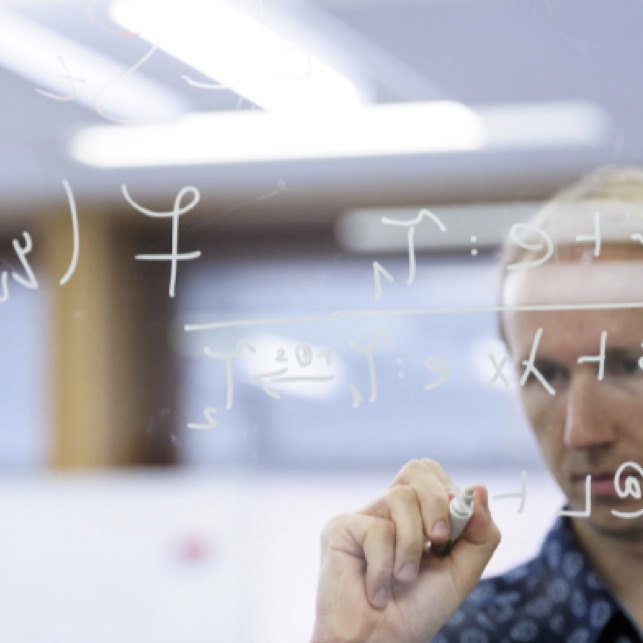
\includegraphics[height=0.65\paperheight,keepaspectratio]{drawing-on-glass.jpg}
			\end{figure}
  		\end{column}
  	\end{columns}
\end{frame}

\section{The Data}
\begin{frame}{Demographic Health Survey (DHS)}
	\begin{columns}[T,totalwidth=\textwidth]
        \begin{column}{0.45\textwidth}
	        \begin{block}{Description}
	           DHS national household surveys conducted in 2015.
	           
	        \end{block}
	        \begin{block}{Usage}
	           Different targets to predict, with the lowest aggregation being the DHS cluster.
	        \end{block}
	    \end{column}
	    
	    \begin{column}{0.55\textwidth}
			\begin{figure}
				\vspace{-\blocktitlesize}
				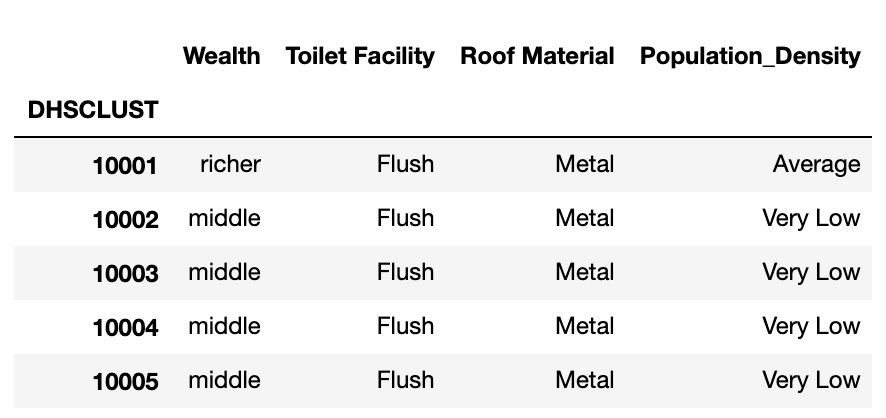
\includegraphics[height=0.45\paperheight,keepaspectratio]{images/dhs.png}
			\end{figure}
  		\end{column}
  	\end{columns}
\end{frame}

\begin{frame}{Open Street Maps}
	\begin{columns}[T,totalwidth=\textwidth]
        \begin{column}{0.45\textwidth}
	        \begin{block}{Description}
	           Open Source geospatial data -----map tiles (geotiff) and vector data
	        \end{block}
	        \begin{block}{Usage}
	           Location about the hospitals, cafe's and colleges.
	        \end{block}
	        \begin{block}{Status}
	         Python modules implemented to use the OSM API to collect vector and geotiff data given a district boundary.
	        \end{block}
	    \end{column}
	    
	    \begin{column}{0.6\textwidth}
	    \begin{figure}
	        \vspace{-3\blocktitlesize}
            \begin{minipage}{.5\linewidth}
                \centering
                \subfloat{\label{main:a}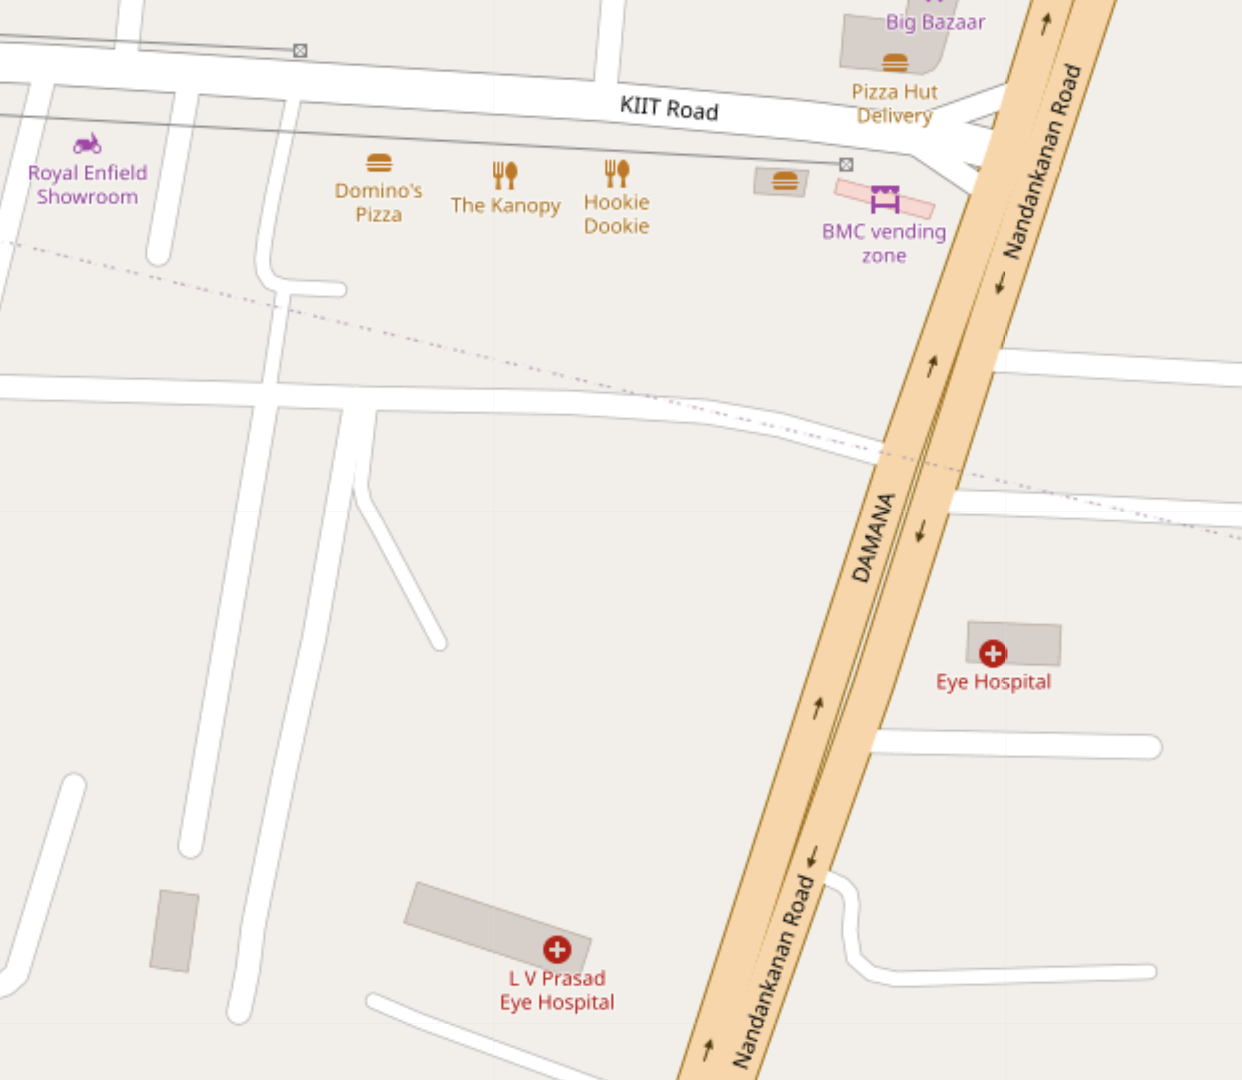
\includegraphics[height=0.36\paperheight,scale=0.6]{images/osm.png}}
            \end{minipage}\par\medskip
            \begin{minipage}{.5\linewidth}
                \centering
                \subfloat{\label{main:b}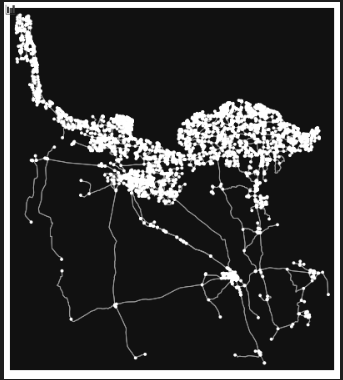
\includegraphics[height=0.36\paperheight,scale=0.7]{images/araria-osm-vector}}
            \end{minipage}
            \label{fig:main}
        \end{figure}
  		\end{column}
  	\end{columns}
\end{frame}

\begin{frame}{Night Time Lights}
    \vspace{-\blocktitlesize}
    \begin{columns}[T, totalwidth=\textwidth]
        \begin{column}{0.45\textwidth}
            \begin{block}{Description}
           NASA's VIIRS/NPP Lunar BRDF-Adjusted Nighttime Lights Daily L3 Global 500m Linear Lat Lon Grid.
            \end{block}
            \begin{block}{Usage}
            To be used as a proxy measure for economic activity
            \end{block}
            \begin{block}{Status}
            Python script to download hdf5 files based on region and time range and convert to geotiff format.
            \end{block}
        \end{column}
        \begin{column}{0.6\textwidth}
            \begin{figure}
                \vspace{-\blocktitlesize}
                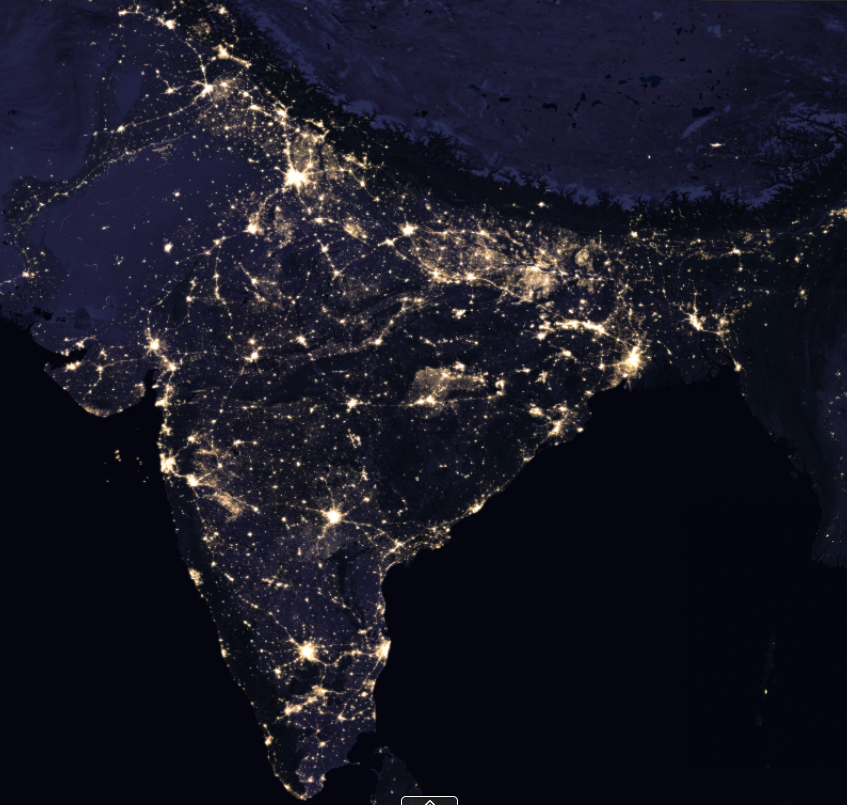
\includegraphics[height=0.65\paperheight,keepaspectratio]{images/india-ntl.png}
                \label{fig:india_ntl}
            \end{figure}
        \end{column}
    \end{columns}
\end{frame}

\begin{frame}{Joining DHS, OSM and NTL data}
	\begin{columns}[T,totalwidth=\textwidth]
        \begin{column}{0.45\textwidth}
	        \begin{block}{Voronoi Polygons}
	        Given a finite set of DHS cluster points the map is divided into cells where each cell covers the region closest to a particular cluster point.
	        \end{block}
	        \begin{block}{Combine DHS and OSM data}
	        Every OSM data point gets the same id as the Voronoi Cell which contains it.
	        \end{block}
	    \end{column}
	    
	    \begin{column}{0.45\textwidth}
			\begin{figure}
				\vspace{-\blocktitlesize}
				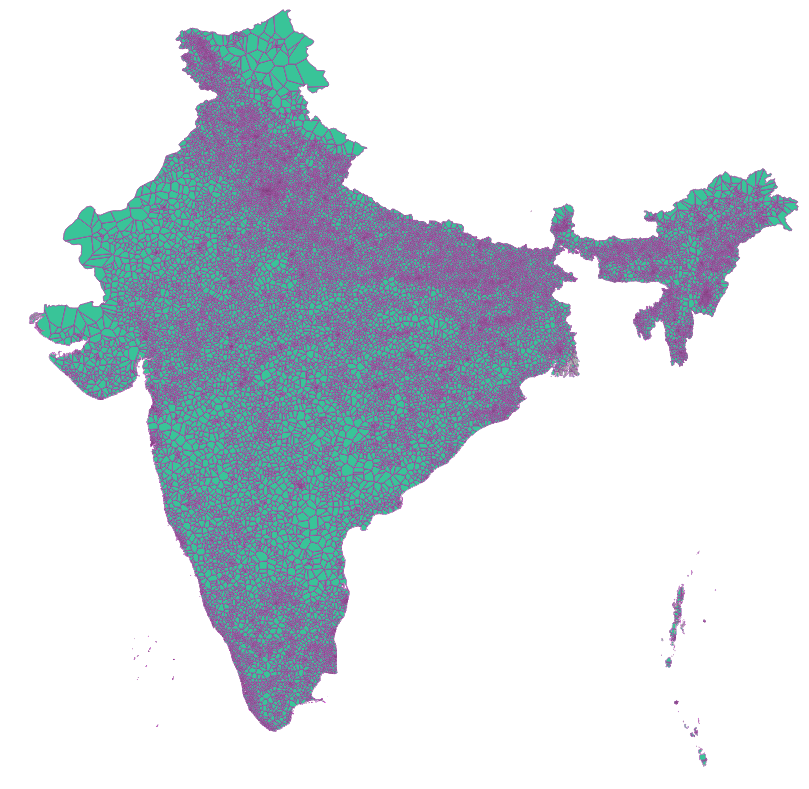
\includegraphics[height=0.65\paperheight,keepaspectratio]{images/india-voronoi.png}
			\end{figure}
  		\end{column}
  	\end{columns}
\end{frame}



\section{Solution}
\begin{frame}{Data Integration}
	\begin{columns}[T,totalwidth=\textwidth]
        \begin{column}{0.45\textwidth}
	        \begin{block}{Description}
	           Integrating all the data in a pipeline:
	           \begin{itemize}
	               \item \textbf{DHS}(Target): Wealth Indicators
	               \item \textbf{OSM}(Features): Describing amenities in the Cluster
	           \end{itemize}
	           
	           
	        \end{block}
	        \begin{block}{Usage}
	           Different targets to predict, with the lowest aggregation being the DHS cluster.
	        \end{block}
	    \end{column}
	    
	    \begin{column}{0.55\textwidth}
			\begin{figure}
				\vspace{-\blocktitlesize}
				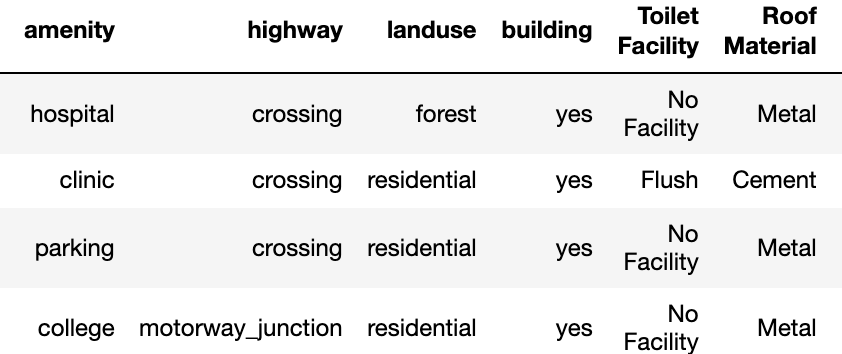
\includegraphics[height=0.4\paperheight,keepaspectratio]{images/dhs_osm.png}
			\end{figure}
  		\end{column}
  	\end{columns}
\end{frame}

\begin{frame}{Modeling}
	\begin{columns}[T,totalwidth=\textwidth]
        \begin{column}{0.45\textwidth}
	       \begin{block}{The label}
	        Mean Absolute Error of 0.64
                \begin{itemize}
                    \item 1:  Poorest
                    \item 2 : Poor
                    \item 3 : middle 
                    \item 4 : richer
                    \item 5 : richest
                \end{itemize}
	       \end{block}
	    \end{column}
	    
	    \begin{column}{0.65\textwidth}
			\begin{figure}
				\vspace{-\blocktitlesize}
				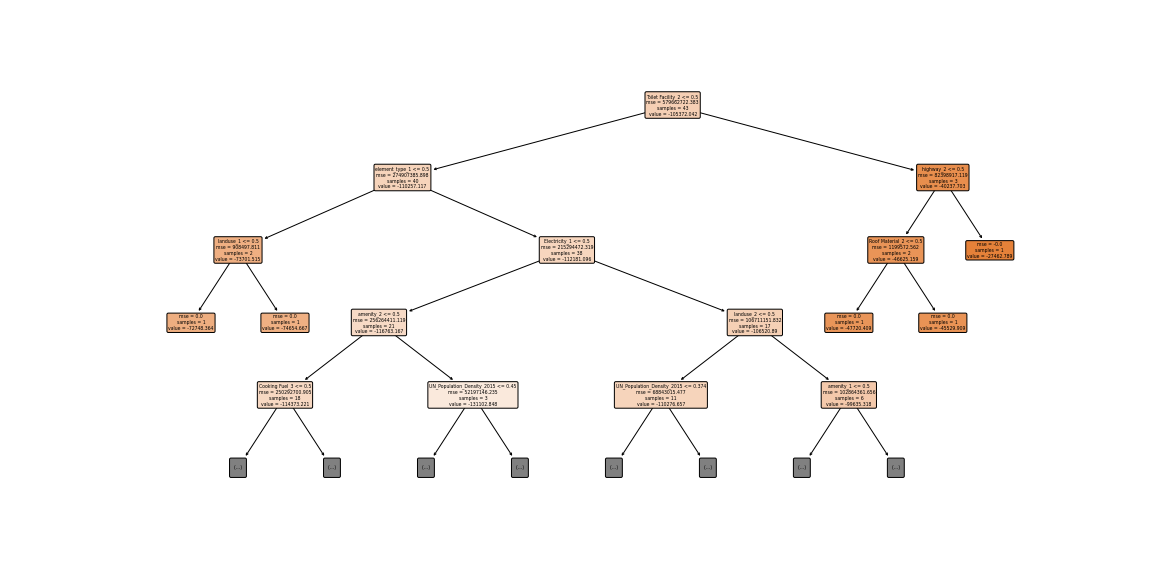
\includegraphics[height=0.5\paperheight,keepaspectratio]{images/tree_ohe.png}
			\end{figure}
  		\end{column}
  	\end{columns}
\end{frame}


\begin{frame}{Modeling}
	\begin{columns}[T,totalwidth=\textwidth]
        \begin{column}{0.45\textwidth}
	        \begin{figure}
				\vspace{-\blocktitlesize}
				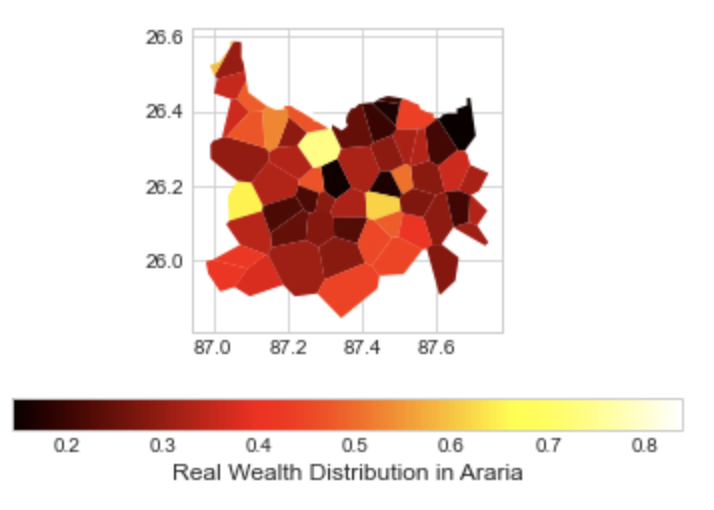
\includegraphics[height=0.45\paperheight,keepaspectratio]{images/real.png}
			\end{figure}
	    \end{column}
	    
	    \begin{column}{0.55\textwidth}
			\begin{figure}
				\vspace{-\blocktitlesize}
				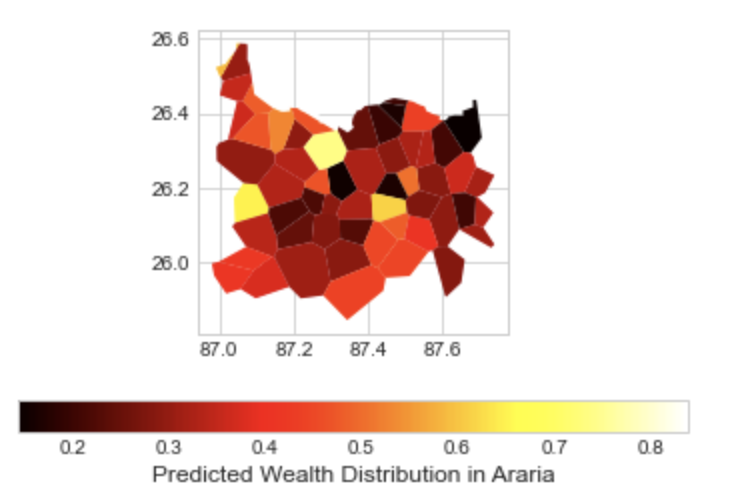
\includegraphics[height=0.45\paperheight,keepaspectratio]{images/preds.png}
			\end{figure}
  		\end{column}
  	\end{columns}
\end{frame}


\begin{frame}{Modeling}
	\begin{columns}[T,totalwidth=\textwidth]
            \begin{figure}
				\vspace{-\blocktitlesize}
				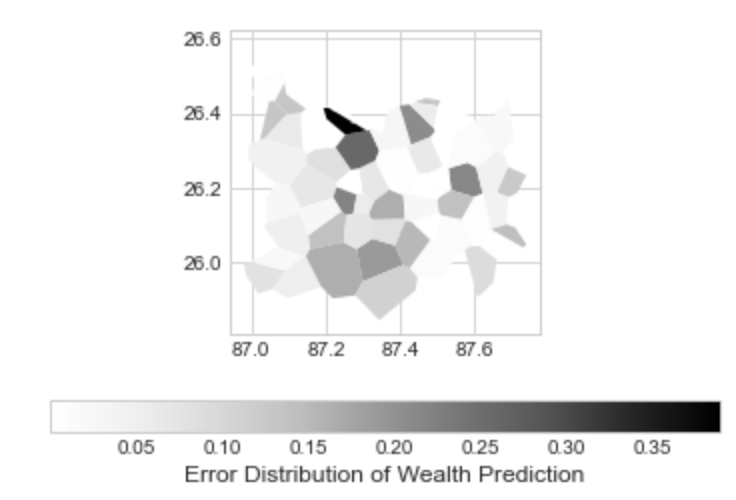
\includegraphics[height=0.65\paperheight,keepaspectratio]{images/diff.png}
			\end{figure}
  	\end{columns}
\end{frame}

\section{Conclusion}

% Skeleton double-column text slide (two text columns)
\begin{frame}{Conclusion}
	\begin{columns}[T,totalwidth=\textwidth]
  		\begin{column}{0.45\textwidth}
  			\begin{block}{Results}
    				Predictive Model that is computationally cheap
    				\begin{itemize}
    				    \item Open Source Data
    				    \item No cloud computing resources
    				\end{itemize}  
			\end{block}
  		\end{column} %
  		\begin{column}{0.45\textwidth}
  			\begin{block}{}
    				Modeling remains explainable and accountable while preserving accuracy
    				\begin{itemize}
    				    \item Explainable and Interpretable machine learning
    				    \item Accountable
    				    \item High Generalization
    				
    				\end{itemize}  
			\end{block}
  		\end{column}%
	\end{columns}
\end{frame}
\begin{frame}{Future Work}
	\begin{columns}[T,totalwidth=\textwidth]
  		\begin{column}{0.45\textwidth}
  			\begin{block}{Steps}
    				\begin{itemize}
    				    \item Scale Up
    				    \item Integrate with NTL
    				    \item Temporal Evaluation
    				\end{itemize}  
			\end{block}
  		\end{column} %
  		\begin{column}{0.45\textwidth}
  		  	\begin{block}{Scope}
    			\begin{itemize}
    			    \item Towards an application?
    			    \item Towards deployment?
    				\item Towards research?
    				\end{itemize}  
			\end{block}
  		\end{column}%
	\end{columns}
    
\end{frame}

\end{document}
